\chapter{Cetacean Detection Using Deep Learning}\label{ch:cetDet}

When building any large-scale project, it is important to break the task down into various subcomponents. In this Chapter we will examine one such subcomponent utilised in the developed automatic photo-id system, the cetacean detector. This component takes images captured during photo-id surveys and detects regions of interest, in our case these are dorsal fins which have breached the waterline. This Chapter will discuss the requirements a detector must meet, how it was trained, how the optimal hyperparameters were found, and how the detector can be utilised to provide a downstream identification system with only the information it needs. 

\section{Requirements of a Cetacean Detector}\label{ch:cetDet,sec:requirements}

Before a system for automatic cetacean detection can be developed, it is important to first define the problem and understand the requirements of the system. The overall aim of the detector is to be able to take large-scale images as input, fed in one at a time, and process them in order to locate regions of interest. Unlike other automated detection systems common in literature, this system is only required to detect one class of object, \texttt{dolphin}. These detected regions can then be passed further down the system pipeline to the identifier. 

 As such, this detector can be considered a coarse-grain task, and at first glance may seem somewhat trivial. However, due to both the nature of the environment in which the class must be detected, and the technical requirements the system must perform under, this becomes a much more complex problem. 
 
 \subsection{Environmental Requirements}\label{ch:cetDet,sec:requirements,sub:environmental}
 
 First the area in which this system is to be deployed, in open water, is susceptible to adverse weather conditions such as high winds. This in turn leads to sub-optimal conditions for detection which the system must be capable of handling, most notably high amounts of sea swell. Further to this, dolphins, the main data subject of this work, are communal and travel in pods. An example of this behaviour can be seen in Figure \ref{fig:pod-eg} Thus, the system must be capable of differentiating between overlapping individuals. Even if not all of the overlapping individuals are suitable for identification down the line, the system must still be able to separate them into individual detections to prevent further misclassification downstream; for example, lets assume an image is inputted to the detector containing three overlapping individuals where one of these has markings clear enough for a human to identify the individual. For our system to also be able to do this, the detector must be able to separate the overlapping animals into the individual components. This allows for the identifier to be provided with three images, one of which is the individual that is identifiable. If all overlapping individuals were passed to the identifier as one, the chance of identification will be greatly reduced, and the image may be identified as \texttt{noise}. 
 
 \begin{figure}
 	\begin{center}
 		\includegraphics[scale=0.06]{Chapter3/figs/dolphins-in-pod-example.JPG}
 	\end{center}
 	\caption{Some cetaceans, such as bottlenose dolphins, travel in pods. The developed detection system must be capable of splitting this pod into individual animals to be passed to the identifier.
 	}
 	\label{fig:pod-eg}
 \end{figure}

 Next, the detector must be capable of differentiating between dolphin fins and waves. Again this might sound trivial, but thousands of years of evolution have resulted in fins and waves looking extremely similar to the untrained eye, which artificial ones often start out as. Especially from a distance and in choppy waters, fins and waves often have extremely similar shape and dimensions. Furthermore, the animal's bodies are also similarly coloured to their surroundings. These adaptations allow the animals to be better protected and camouflaged in their environment, but can cause issues with detection systems. This becomes apparent when thinking about how CNNs \textit{see}. As described in Chapter \ref{ch:Background,sec:DLforCV}, CNNs see input images as a matrix of pixel values. When training an object detection system, the CNN is also told which parts of this matrix are related to a class, any without a class label are considered background. If fins and areas of background contain similar pixel values, and these pixel values are clustered in the same ways, this can result in issues when training a model to detect instances of a class without misclassifying the background. 
 
 Another important requirement is for the detector to be able to handle objects of varying size, shape, direction, and angle of approach to the camera. When working in an open water environment with live animals, the conditions that you will capture images of the animal under are extremely variable. You may capture an image of the animal at any point in it's breaching process, which will change the size of the dorsal fin which is above the waterline. As dorsal shape is unique to each individual, the detector must be capable of understanding a general `fin-shape' rather than a fixed one. 
 
  \begin{figure}
 	\begin{center}
 		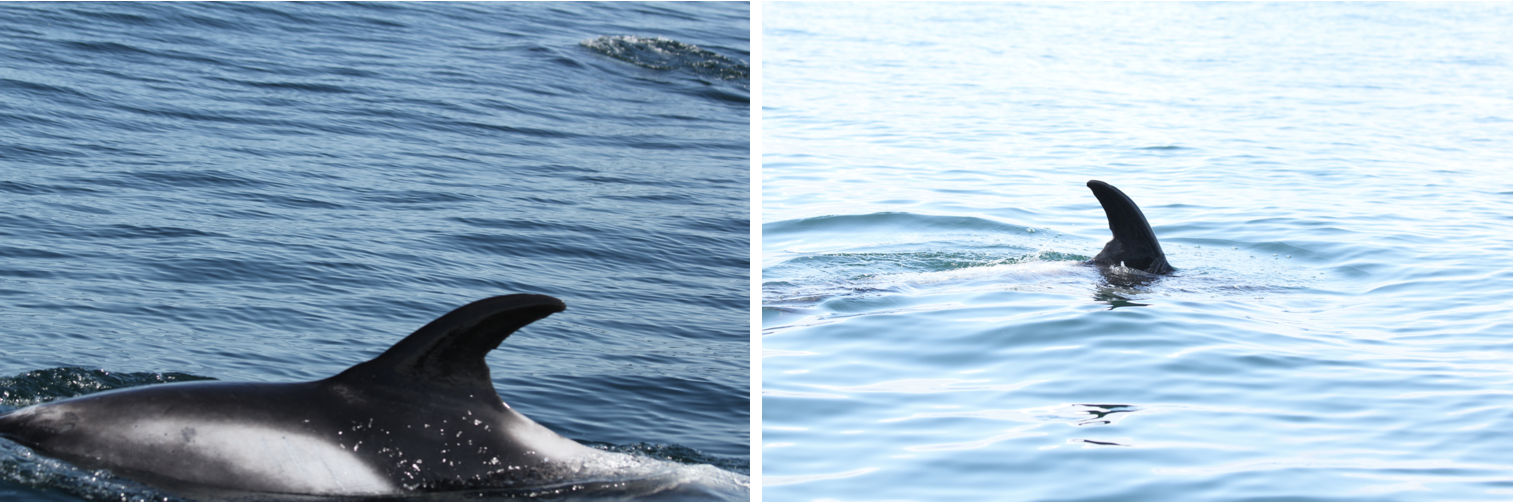
\includegraphics[scale=0.6]{Chapter3/figs/angle-size-example.png}
 	\end{center}
 	\caption{Two images of the same individual taken from different angles of approach, directions of travel, and distances from the vessel. Note how this changes the make-up of the dorsal fin, however keeps the identifying notch visible. 
 	}
 	\label{fig:angle-eg}
 \end{figure}
 
 Furthermore how the animals breach the waterline is also extremely variable. Breachings may occur at any  direction relative to the boat and the animal could itself be travelling in a different cardinality. The ideal scenario in this case would be for a breaching to occur either directly East or West of the boat (off the port or starboard side respectively) and for the animal to be travelling perpendicular as this provides the best chance of mark capture, however this rarely occurs. For example, a breaching may occur off the port-side of the bow (approx North West relative to the boat), but the animal may be travelling in a South-Easterly direction. These approaches greatly change the look of the fin, however they may still contain identifiable markings, thus our detector should be able to detect these fins and pass them along for identification. An example of this can be seen in Figure \ref{fig:angle-eg}, which also shows how distance from the vessel can change the camera's view of the dorsal. 
 
 As mentioned previously, weather conditions can also greatly affect how a dorsal fin is captured by a camera. However, especially in mark-recapture surveys, there are only two conditions that need to be worried about; swell and lighting, other conditions do not need to be handled by this detector. This is due to most research groups having limits of sea state for safety reasons. With regards to Newcastle University's Marine MEGAfauna Lab, this limit is a sea state less than 3 on the Beaufort scale \cite{world_meteorologicial_society_beaufort_1970}. As such a mild amount of swell and splash can be expected, which the detector should be capable of handling. Lighting conditions are not considered in the Beaufort scale, but for operational reasons the vast majority of mark-capture surveys take place during daylight hours. This can lead to large amounts of glare in images, especially on clear days. As such, the detector should be invariant to these conditions. 
 
 \subsection{Technical Requirements}\label{ch:cetDet,sec:requirements,sub:technical}
 
 As well as being able to handle a variety of environmental factors, there are also some technical requirements that the detector must meet. With all deep learning based computer vision approaches, there is often a trade off that must be made between speed and accuracy. In most cases, these are inversely proportional to each other; the faster a system is required to perform, the lower an accuracy you must be willing to tolerate - Huang \textit{et al.} discuss this in greater detail in their 2017 paper \cite{huang_speedaccuracy_2017}. Thanks to the pace of research in this area, 2020 saw the release of object detection architectures which can perform operations in real-time such as EfficientDet \cite{tan_efficientdet_2020} and YOLOv4 \cite{bochkovskiy_yolov4_2020}. Current results on benchmark datasets using these real-time architectures are still a long way off their non-real-time competitors however, and accuracies would drop further on custom non-benchmark tasks such as cetacean detection. 
 
 Because this trade off must be made, before deploying a deep learning model it is important to decide where the system will be utilised. As photo-id surveys are performed on small vessels such as RIBs, space is severely limited on board. Because of this, it is not appropriate to add additional hardware to the vessel to perform this analysis during the survey. Furthermore, the current methodology of cetacean researchers is to perform identification once back on land, even when utilising photo-id aides. As the system proposed in this project is intended to fit into existing procedures rather than replace researchers, it is appropriate for the system to also be land based rather than on the vessel. Thinking about the current procedure further, this project's proposed system could be, for example, left running overnight performing identifications whilst the researchers are away or during the day whilst they are on surveys, being left to work through the last day's worth of images captured. As such, there is no need for the system to operate in real time to fit in with the current workflow of cetacean researchers, provided the system completes its task within a reasonable time frame. Further to this, as the output of the detection model will be passed to an identification module, it is imperative that as much noise is removed as possible during the detection. In order to do this, the accuracy of the detection must be as high as possible, furthering the case for an accurate system over a fast one.
 
  This idea of reducing as much noise as possible can be used to further narrow down the requirements of the detection system. As discussed in Section \ref{ch:Background,sec:DLforCV}, the output of detection systems can be provided in different formats. In bounding box detection systems the detected objects are denoted by a set of at least two pixel coordinates denoting the top-left and bottom-right extremes of the object. These detections are often more cost-effective, both from a labelling perspective requiring less person-hours to complete, and to perform computationally. However, a model trained on bounding boxes will produce outputs which will only partially remove noise deemed to be outside of the detection's extreme points.
 
 If we utilise pixel wise mappings however, then each pixel is given a classification. This allows the system to be more discrete with its detection, telling us exactly where the object is in the image. These pixel locations can then be used to removed all background. Pixel wise labelling is far more labour intensive however, and thus more financially costly to produce. Both semantic and instance segmentation methods will allow the detector to utilise pixel-wise mappings to remove background noise. However, utilising our requirement defined earlier in Section \ref{ch:cetDet,sec:requirements,sub:environmental} that the detector must be capable of reducing an overlapping pod to its individual component animals, requiring the use of instance segmentation in any pixel-wise detections would be preferred. 
 
 As such, this requirement reveals a further trade-off the system must make. The amount of noise removed by the detector is proportional to the cost and labour needed to create data to train the system; this was required to be explored in more detail before it could be decided if bounding boxes or instance segmentation masks would be more appropriate for use with the detector. This is discussed in more detail in Section \ref{ch:cetDet,sec:deciding,sub:boundingBoxInvestigation}.
 
 Furthermore, any system performing cetacean detection must be capable of working with large scale images. In most image based tasks where deep learning is utilised images fed to the network are downscaled, typically to sizes such as 224x224 to allow for faster training and a reduction in overall network size. Downscaling images reduces the number of pixels in the image, which by definition reduces the amount of information present as pixels values need to be pooled (one pixel needs to now display what multiple would have previously). For most detection tasks this would not be an issue, and indeed if this project was solely a cetacean detection task there would be no issues with downscaling. This detector is not stand-alone however but rather the first stage of a pipeline of networks with the end goal of photo-identification. The identification task relies on potentially minute details in the fin such as notches; any downscaling of the image at the detection stage runs the risk of removing potentially identifiable information in the fin. As such, the image must only be reduced in size once it is certain that no identifying information will be lost. As this cannot be guaranteed at the stage of detection, the detector must be capable of operating on images without resizing.
 
\section{Deciding on Architecture and Framework}\label{ch:cetDet,sec:deciding}

Based on the requirements outlined in Section \ref{ch:cetDet,sec:requirements}, it is possible to begin deciding on how the cetacean detector is to be developed. One of the most important factors in the overall approach taken in the detector's development would be its use of either bounding boxes or pixel-wise mappings during training. As mentioned previously, the use of pixel-wise mappings would allow for a greater removal of background noise, but is extremely costly and labour intensive to produce. In contrast, bounding box labels are easier and cheaper to produce but will lead to less background noise removal. 

\subsection{An Investigation into Bounding Boxes}\label{ch:cetDet,sec:deciding,sub:boundingBoxInvestigation}

Due to their relative cheapness and ease to produce, the use of bounding boxes in this project would be extremely beneficial. However, if the use of bounding boxes at this stage would hinder the accuracy of individual identification downstream, then this would outweigh the cost of pixel-wise mappings. 

As such, an investigation was undertaken to decide whether bounding boxes would be a viable option, and if their use would hinder downstream identification. To begin, a small amount of data was provided by the Marine MEGAfauna Lab, discussed in more detail in Section \ref{ch:cetDet,sec:initialTesting,sub:zanzibar}, which contained images captured during a previous cetacean survey. A subset of this data was manually cropped to simulate the output of a bounding box detector, an example of which can be seen in Figure \ref{fig:manual-crop-example}. This manually cropped data included some background but ensured the region of interest, the dorsal fin, was centred and prominent, representing an optimal output from a bounding box detector. 

\begin{figure}
	\begin{center}
		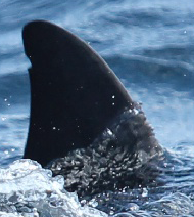
\includegraphics[scale=0.6]{Chapter3/figs/manual-crop-example.png}
	\end{center}
	\caption{An example manual crop utilised in bounding box suitability testing.
	}
	\label{fig:manual-crop-example}
\end{figure}

\subsubsection{Feature Extraction with SIFT}\label{ch:cetDet,sec:deciding,sub:boundingBoxInvestigation,subsub:SIFT}

To begin, processing of the cropped images focussed on the use of feature extractors such as Scale-Invariant Feature Transform, also known as SIFT \cite{lowe_object_1999}. As the name suggests, SIFT is invariant to scale, a major advantage for use with cetacean survey data where the region of interest's size may change depending on when the image of the dorsal fin breaching the water is captured. If SIFT was capable of producing feature descriptors of the dorsal fins with only partial background removal, this would show potential for individual identification where some background is present, possibly through the use of the feature descriptors. 

First SIFT was performed on the entire cropped image, however this proved unfruitful, picking out very few features in areas of the image which contained the animal's dorsal fin and instead focussing on the feature heavy areas present in the sea, even in images containing relatively calm water. This result indicated that further refinement was required, potentially reducing the area SIFT was allowed to explore. 

Reduction of the search space available to SIFT was achieved through the use of colour thresholding. Here, a mask was created programmatically for each image based on bounded RGB colour values found in the dorsal fins, giving an upper threshold of (14, 16, 26) and a lower threshold of (54, 51, 66). As such, SIFT would only be performed in areas of the image where pixel values fell within this range. An example result of SIFT after colour thresholding can be see in Figure \ref{fig:manual-crop-sift-colour-thresholding-example}, with coloured circles surrounding an extracted feature. As can be seen, colour thresholding helps in removing a large amount of background water from the computation. However, issues arise where areas of water are also within this thresholding. Because of this, colour thresholding before SIFT only reduces the amount of features extracted from the water, it does not remove them, which may result in misidentification downstream.

Further to this, it can be seen that SIFT is incapable of extracting relevant features used in the photo-id process. For example, in Figure \ref{fig:manual-crop-example}, a notch is clearly present on the dorsal fin which would be a good marker for individual identification. However, when performing SIFT on this dorsal as seen in Figure \ref{fig:manual-crop-sift-colour-thresholding-example}, note how this feature has not been detected by SIFT, which has instead detected an area above the notch which contains no identifiable information. 

\begin{figure}
	\begin{center}
		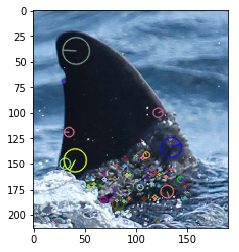
\includegraphics[scale=0.6]{Chapter3/figs/manual-crop-sift-colour-thresholding.png}
	\end{center}
	\caption{An example manual crop showing the result of SIFT feature extraction when thresholded based on RGB colour values.
	}
	\label{fig:manual-crop-sift-colour-thresholding-example}
\end{figure}

Feature extraction methods such as SIFT are also incapable of extracting other identifiable markers such as fin shape. As such, the use of SIFT was deemed improper for this use case. It is important to note here that the use of SIFT may be appropriate for cetacean species other than this project's data subjects of bottlenose and white-beaked dolphins. For example, the use of SIFT has been shown to be appropriate to aid in identification of individual Risso's dolphins \cite{reno_sift-based_2019}.

\subsubsection{Background Removal with GrabCut}\label{ch:cetDet,sec:deciding,sub:boundingBoxInvestigation,subsub:GrabCut}

Testing the suitability of SIFT as described in Section \ref{ch:cetDet,sec:deciding,sub:boundingBoxInvestigation,subsub:SIFT} highlighted the need for complete background removal before identification would be possible with bottlenose and white-beaked dolphins. In order for bounding boxes to be a viable option in this scenario, a robust background removal process would need to be created. Further, the process would need to be capable of operating under unseen conditions in an unsupervised manner without labelled segmented  data to train on. If the background removal process required training data to operate, this would increase the overall cost and labour required to use bounding boxes, and as such reduces the suitability of them compared to utilising pixel-wise mappings from the beginning. 

The current state of the art in this area is GrabCut, proposed by Microsoft Research \cite{rother_grabcut_2004}. This algorithm allows for the segmentation of foreground objects from the background with minimal or no human interaction. As GrabCut would be utilised in a fully automated setting, GrabCut would be required to perform background removal with no human interaction. Testing of the suitability for GrabCut was performed using the same cropped images as those used for SIFT testing. Again, issues arose when performing GrabCut on the cropped image data. The algorithm struggled to understand which parts of the image were classed as background and foreground, which resulted in imperfect segmentations. This was especially an issue where the dorsal fin was present in rough water, where splash would be in-front of the dorsal fin when captured by the camera. The use of GrabCut on Figure \ref{fig:manual-crop-example} can be seen in Figure \ref{fig:grabcut-example}.

\begin{figure}
	\begin{center}
		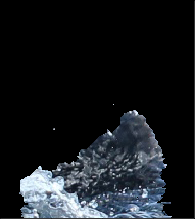
\includegraphics[scale=0.6]{Chapter3/figs/grabcut-example.png}
	\end{center}
	\caption{An example manual crop showing the result of GrabCut background removal.
	}
	\label{fig:grabcut-example}
\end{figure}

As can be seen, the use of GrabCut as a background removal tool does not perform as expected on data the detector is required to operate on. Because of this, as well as the unsuitability of feature extraction as seen in Section \ref{ch:cetDet,sec:deciding,sub:boundingBoxInvestigation,subsub:SIFT}, the use of bounding boxes in the cetacean detector stage was deemed not to be possible. As such, the focus of testing moved to the use of pixel-wise mappings and instance segmentation.  

\subsection{Instance Segmentation Architectures}\label{ch:cetDet,sec:deciding,sub:instanceSegArchitectures}

One of the major decisions that must be made here is which model architecture should be utilised in order to provide the required pixel-level detections. As this project is devoted to improving existing procedures and introducing deep learning to a novel space, it is far more advantageous to utilise existing model architectures rather than develop a custom one. The development of a custom architecture for this stage of the project would be extremely time consuming, taking away time from more novel parts of the project (notably the identification of the individual animals). Further, as this project is introducing deep learning methods to a novel space, the project needs to be able to convince researchers in this space that the system is reliable; this is more easily achieved using a pre-existing architecture where use cases already exist in literature and business. 

To this end there are two main model architectures that can be chosen for this task; U-Net \cite{ronneberger_u-net_2015} and Mask-RCNN \cite{he_mask_2017}. Both of these architectures work in different ways. Vuola \textit{et al.} provide a more detailed comparison between the two models \cite{vuola_mask-rcnn_2019}, however the main focus for this project is their resultant output mask structure. 

U-Net is based on an encoder-decoder architecture. This allows for fast and simple segmentation when working with images where you only require one output. For example, taking U-Net's original use case of biomedical imaging, let's assume we have an image showing a group of cells and we wish to segment them into the individual components. U-Net is able to perform this operation efficiently through boundary estimation to locate the outer edges of the cells which allows them to be segmented from each other. However this results in an output of the same dimensions as the input, that is, all segmentations are provided in a single binary mask. 

In contrast, Mask-RCNN utilises a multi-stage architecture (described in more detail in Section \ref{ch:Background,sec:instanceSegmentation,sub:Mask R-CNN}). This allows the architecture to place each detection on its own binary output mask. This is extremely important for our use case; as our detector will be used as part of a larger system, passing information downstream to the identifier which will require individuals to be in their own images, processing each individual in series. If U-Net was utilised for the detection stage, whilst initially being more efficient than Mask-RCNN, further processing of the binary output mask would be required to split this into it's individual components. In contrast, if Mask-RCNN was utilised then the processing required in between the detection and identification stage would be far simpler. Again, this allows for more time to be spent working on the novel aspects of this project whilst keeping the pipeline as simple as possible. This reason was a big factor in deciding to focus on Mask-RCNN for this stage.

Another factor which must be decided upon when starting developing a deep learning system is the language and framework to be used for development. With regards to language this was a fairly simple decision; the vast majority of deep learning research and development is written in Python. The language benefits from an efficient and lightweight syntax as well as having a host of different deep learning packages available to aid in development. Further to this, both of the major deep learning frameworks, Google's Tensorflow \cite{abadi_tensorflow:_2016} and Facebook's Torch (of which PyTorch is the most actively developed) \cite{paszke_automatic_2017}, both provide full Python support and have active communities for the language. Thanks to this, the vast majority of deep learning development is performed using Python in one of these two frameworks. By utilising these technologies, this project's code is easily reproducible and understood, as well as extendable in the future.

Of the two main frameworks, the use of Tensorflow was decided for this project. Whilst this decision was made somewhat due to personal preference, Tensorflow was (at least at the time of starting this project) the primary framework for development of deep learning systems outside of academia. Rather than developing a custom Mask-RCNN in Tensorflow for this project, Matterport's Mask R-CNN implementation \cite{waleed_mask_2017} has been adapted. Whilst this does require the use of an old version of Tensorflow (1.14), this version is also stable and has a large library of available support unlike the most recent versions (>= 2.0).

\section{Initial Testing of Mask-RCNN}\label{ch:cetDet,sec:initialTesting}

In order to build a Mask-RCNN detector which fulfilled the requirements as laid out in Section \ref{ch:cetDet,sec:requirements} an understanding of the framework needed to be achieved. Thankfully, the downloaded repository also includes some tutorial notebooks, most notably an example on balloon segmentation which proved invaluable for learning the basics of how Mask-RCNN operates both on a fundamental code level and at a higher level, understanding how the code can be adapted for other use-cases. In order to progress onto cetacean detection however, a dataset of cetaceans would be needed. 

Exploration of available open-source datasets to find cetaceans in conditions this detector would be operating in proved unfruitful. Many standard benchmarking datasets contain animal classes, and thus an exploration of these was conducted. Of the more generalised benchmark datasets, those such as ImageNet \cite{deng_imagenet:_2009} which contain a large corpus of varied classes, only CIFAR-100 \cite{krizhevsky_learning_2009} contains a \texttt{dolphin} class. However, images in CIFAR-100 are only 32x32 pixels in size, too small to be useful for the task at hand. 

Moving the search away from generalised datasets and towards those which are targetted at conservation efforts or the natural environment also proved fruitless. A large portion of these datasets focus on camera traps or land-based fauna, such as iWildCam \cite{beery_iwildcam_2019}, for reasons discussed in more detail in Section \ref{ch:Background,sec:conTech}. Some images included in the iNaturalist dataset \cite{van_horn_inaturalist_2018} are of cetaceans, such as a class for the short-beaked common dolphin (\textit{Delphinus delphis}), however most focus on other aquatic animals such as the Florida manatee (\textit{Trichechus manatus}), various amphibians, and molluscs. 

\subsection{The Zanzibar Dataset}\label{ch:cetDet,sec:initialTesting,sub:zanzibar}

Due to the lack of open-source and published datasets to aid in the development of this cetacean detector, one was required to be created. As the focus of this project as a whole was the utilisation of the developed system to aid in conservation efforts of resident cetacean populations off the Northumberland coastline, ideally the created dataset would come from this area. At the time of initial testing however this was not possible due to a lack of available data from the survey area.

As such, alternative data was provided by the Marine MEGAfauna Lab. The dataset was curated during a 2015 conservation effort undertaken in Zanzibar, Tanzania, to determine the status of Indo-Pacific bottlenose dolphins (\textit{Tursiops aduncus}) in the area \cite{sharpe_indian_2019}. The catalogue provided consisted of 1021 images of size 5184x3456, and was supplied in a format suitable for manual photo-identification rather than for the training of a neural network. Work was then undertaken to convert this conservation catalogue into a machine learning dataset. 

In order to convert this catalogue into a machine learning dataset, the provided images must first be labelled. This was achieved using the VGG Image Annotator software, known as VIA \cite{dutta_via_2019}. Other labelling software such as LabelImg \cite{tzutalin_labelimg_2021} were examined, however VIA was deemed the best choice for the task at hand. This software was chosen for multiple reasons; first, the software is noticeably easy to use and allows for efficient labelling on a per-pixel basis as required by Mask-RCNN. Second, the tutorial data provided by the Mask-RCNN Github repository was labelled in VIA format, showing that this code implementation would accept data labelled in this format. Furthermore, use cases of VIA being utilised for labelling of marine-oriented data are available in literature \cite{nita_cnn-based_2020}, providing evidence of suitability of the labelling software for research purposes and data representing similar conditions.

Before labelling the Tanzania data, some curation was performed. Each image labelled by VIA is required to contain at least one non-background class. As such, any images provided which did not contain an example of a \texttt{dolphin} class were discarded. Other images where the class examples were unsuitable for training a Mask-RCNN model, such as those which contained only an extremely small section of the photographed dolphin or were deemed too blurry, were also removed. This left 312 images which were suitable for the Mask-RCNN.

The process for labelling the data with VIA is rather straightforward. The software runs locally through a web browser, with each image labelled sequentially. Figure \ref{fig:via-json-example-zanzibar} shows an example image labelled using VIA and the resulting JSON created for the image. Each image is shown on-screen to the user who is then able to trace around class examples by selecting multiple points on the image. Once a full trace has been performed, any pixels inside of the trace are treated as one class. This class is labelled through the use of a class attribute, in the case of the Tanzania data this was the class label \texttt{fin}, denoting the class example as a fin above the waterline. These labels are stored in a corresponding JSON file, which is fed to the Mask-CNN model along with the images during training. This labelling allows the model to learn per-pixel class examples during training. This tracing method also allows for each distinct individual in a group to be labelled individually, even if overlapping, which would be much harder to perform with bounding box labelling and allows the model to learn how to differentiate between group members.  

  \begin{figure}
	\begin{center}
		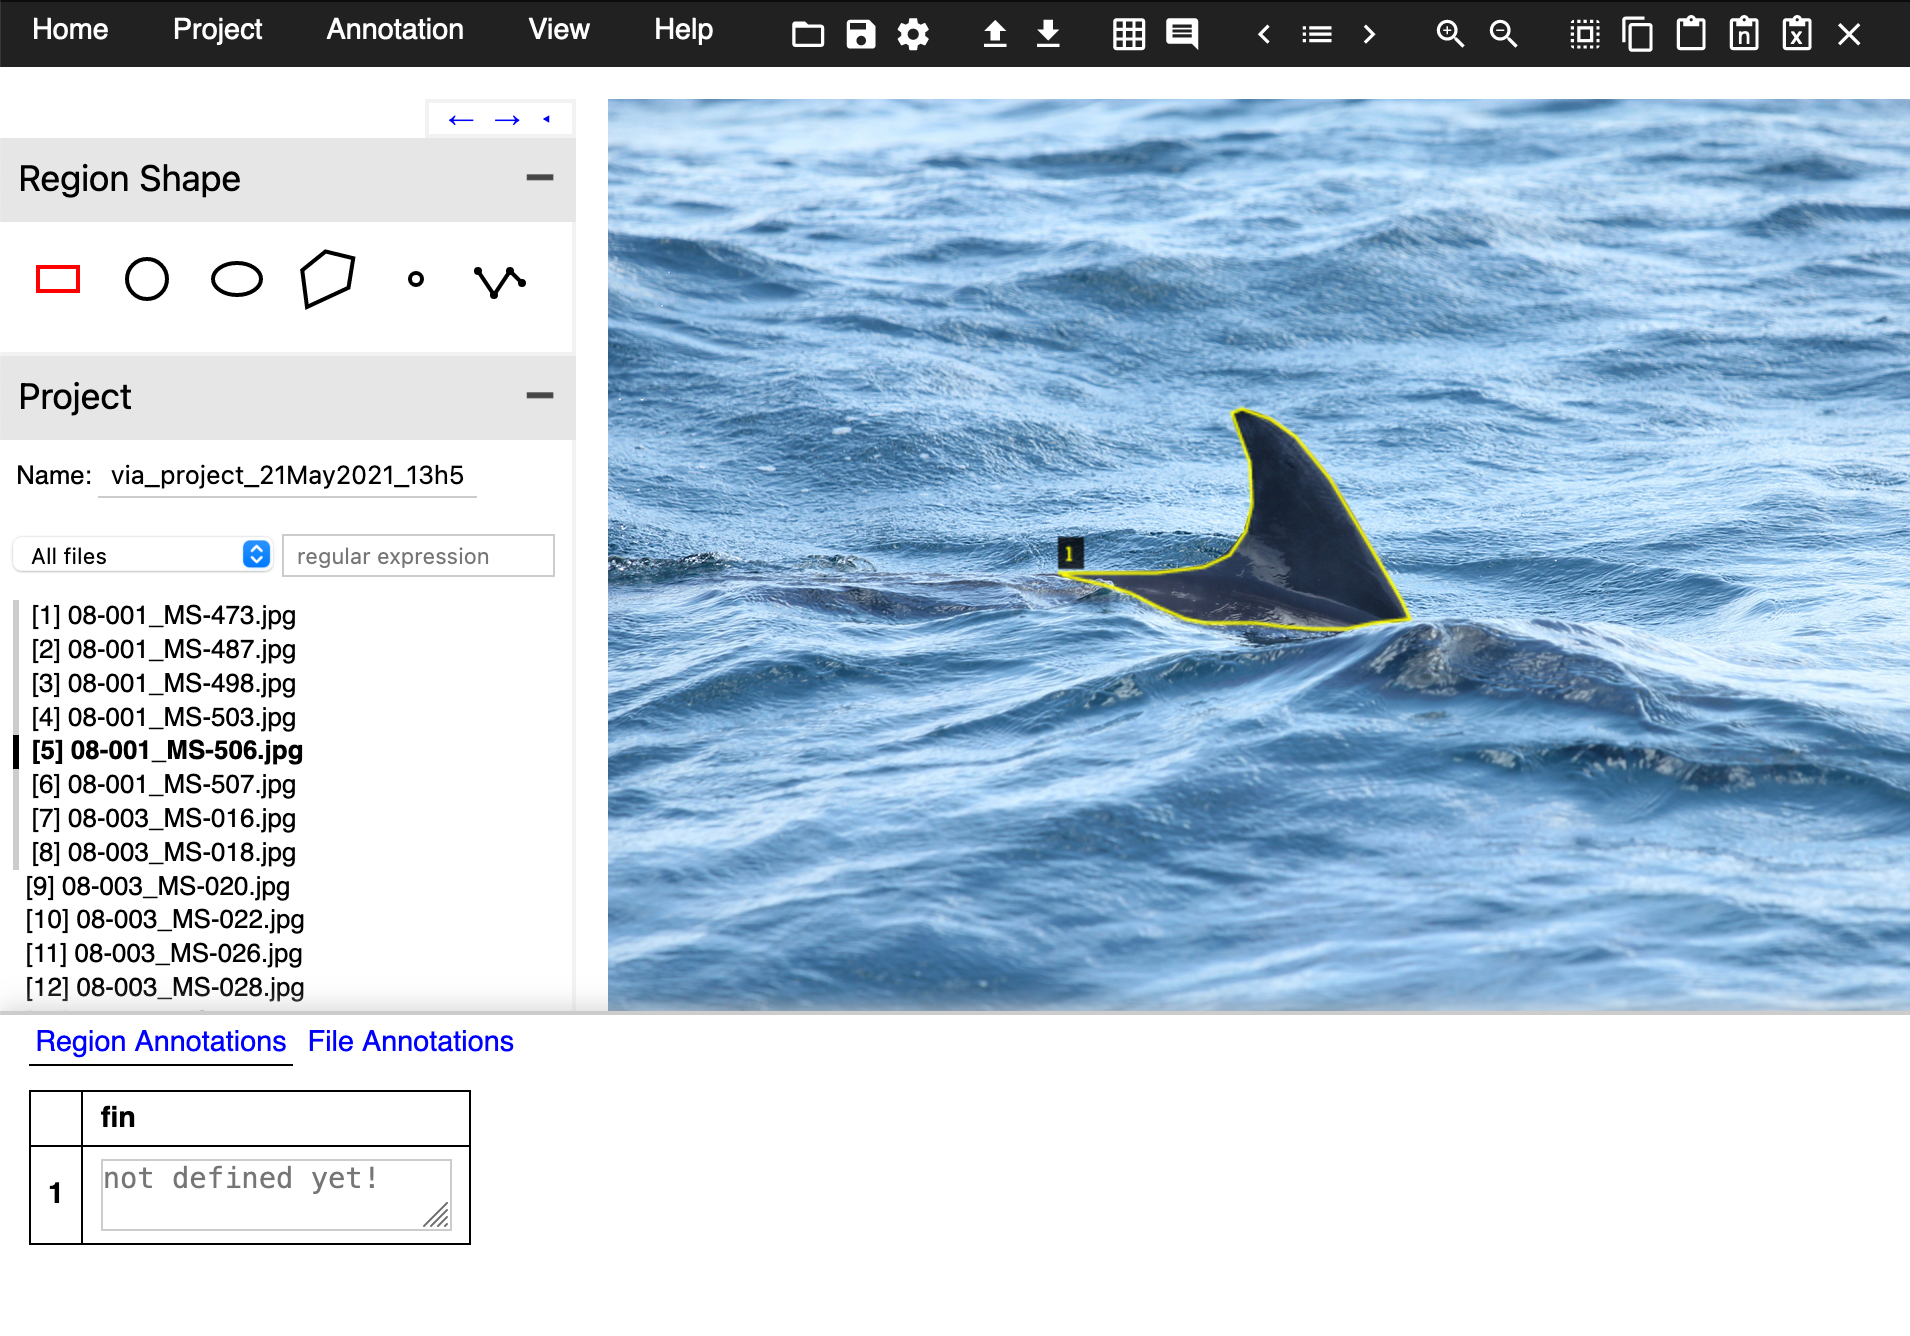
\includegraphics[scale=0.4]{Chapter3/figs/via-json-example-zanzibar-1.png}
	\end{center}
	\caption{An example image showing the labelling processes using VIA.
	}
	\label{fig:via-json-example-zanzibar}
\end{figure}

Once all 312 images had been labelled, it was then possible to create a train-test split. The 312 images were divided using an 80-20 split, where 80\% of the images are designated for training the Mask-RCNN model, known as the training set, and the remaining 20\% were held back for model evaluation, known as the test set. By evaluating on previously unseen data this affords researchers the ability to understand the generalisability of the trained model, mitigating overfitting. 

This newly created Zanzibar dataset would allow for prototyping to begin, determining the suitability of a Mask-RCNN based model for the task of a cetacean detector. The Zanzibar dataset was very similar in content to what would be expected from a dataset created from North Sea survey data once this had taken place and thus gave a good baseline for experimentation. 

\subsection{Transfer Learning}\label{ch:cetDet,sec:initialTesting,sub:transferLearning}

Whilst the Zanzibar dataset provides experimental data similar to that which the Mask-RCNN model will be required to process, the amount of data is extremely small. Deep learning models often require thousands of images when training to produce generalisable and accurate models. As such, this dataset alone would not be enough to train the cetacean detector. One way to fix this issue would be to locate more photo-id data. However, little extra data was readily available from the Marine MEGAfauna Lab, and data from other labs would require a large amount of effort to obtain. Cetacean catalogues are closely guarded by conversation labs due to the large amount of effort required to obtain them. Second, any further data collected would also need to be labelled and incorporated into the now existing dataset, which again would require significant time and effort. These issues rendered the prospect of expanding the Zanzibar dataset unachievable in the time required. 

Another available fix for this issue is the concept of transfer learning. This is a technique whereby models trained to perform one task are repurposed to aid in a second, usually more specialised task. These initial models have typically been trained on large generalised datasets such as ImageNet \cite{deng_imagenet:_2009} or Microsoft's Common Objects in Context, more commonly known as MSCOCO \cite{lin_microsoft_2014}. These datasets often contain hundreds of thousands of images covering a large number of classes, which make them perfect for the task of transfer learning. 

By first training a model on these large datasets, the model is able to learn the basics of image understanding, for example the concept of basic shapes and colour, allowing for the development of a generic visual understanding model. By utilising these models, we effectively provide our own model with a head-start in its learning process, there is no need to utilise the small amount of data available in the Zanzibar dataset for low level learning; it can instead be saved for allowing the model to understand and generalise to the domain specific task, such as cetacean detection. For a more in-depth analysis of transfer learning, see Pan \textit{et al.} \cite{pan_survey_2010}.

Training a neural network, or model, is extremely computationally and time expensive due to the large dataset sizes used. As such, many models suitable for transfer learning can be obtained in a pre-trained state. These pre-trained models are hosted by model zoos, which provide frozen model weight files in a format which allow for transfer learning to take place through a process known as fine-tuning. Here, a model from the zoo is downloaded and \textit{n}-number of deeper layers are unfrozen. Next, additional layers are added to the model which perform the domain specific task. The unfrozen layers and the additional layers are then trained on the domain specific task, allowing for the fine-tuning of the higher-level feature extraction. 

\subsection{Utilising Transfer Learning to Train the Mask-RCNN}\label{ch:cetDet,sec:initialTesting,sub:transferLearningforTheDetector}

The use of transfer learning can be easily adapted for the training of the cetacean detector for use with the Zanzibar dataset, achieved directly through Tensorflow. First, a backbone model is chosen. For the cetacean detector, it was decided that a ResNet50 backbone would be utilised. Matterport's Mask-RCNN implementation allows for the use of a ResNet50 or ResNet101 backbone, both standard variants of ResNet which are 50 and 101 layers deep respectively. ResNet50 was chosen over ResNet101 as during initial experimentation with the Matterport provided tutorial data, no significant improvement in accuracy was achieved using the deeper 101 layer model however this greatly increased training time as double the number of layers were required to be trained. 

Once a backbone has been chosen, it is then loaded into Tensorflow. Next, the pre-trained model weights are downloaded from the model zoo. These weights denote the strength of the connections between the model's layers, and when Tensorflow initially loads in the backbone model the weights of each layer are randomly initialised. During a normal training run, where the backbone model is trained from scratch, these randomly initialised weights would be manipulated through the use of backpropagation; the weights of each neuron in the layer changed to reflect how much effect said neuron has on the output of the layer in order to achieve the desired overall model output (such as a pixel classification). 

In transfer learning however, these initial weights are overwritten by those downloaded from the model zoo. This replicates the state of the model trained on the larger dataset onto the initial backbone model; all of the weights are frozen into their final pre-trained state. As previously mentioned, there are multiple different models available in the zoo usually trained on large benchmark datasets. As such, before utilising transfer learning it is important to make an informed decision about which benchmark dataset the pre-trained model has itself been trained on. For this project it was decided that the ResNet50 weights trained on MSCOCO would be utilised. This was due to the fact that MSCOCO is primarily an instance segmentation dataset, and thus one of the most appropriate to use for transfer learning to another instance segmentation task. The use of MSCOCO for pre-training on Mask-RCNN has in recent years been well documented in literature for a variety of tasks \cite{yu_fruit_2019, couteaux_automatic_2019, fujita_fine-tuned_2020}. When utilising an MSCOCO pre-trained backbone for a Mask-RCNN based task, it is important to note that certain layers must be excluded when loading in the pre-trained weights as these are only utilised in Mask-RCNN models, such as those which deal with the per-pixel masks. This is because these layers require a matching number of classes; if the MSCOCO weights were utilised here there would be a mismatch between the number of classes in MSCOCO (80) and in the Zanzibar dataset (1).

Once the backbone model has been loaded with pre-trained weights, the total number of layers to fine-tune must be decided. This can be considered similar to a hyperparameter, as it must be chosen at run time by the user. Whilst any number of the layers can be chosen for fine-tuning, generally either all of the model layers or only the heads; these are layers required for the Region Proposal Network, the pixel classification, and masking layers of the model. For the purposes of hyperparameter tuning, the number of unfrozen layers can be included in a grid search.

\subsection{Data Augmentation}\label{ch:cetDet,sec:initialTesting,sub:dataaugmentation}

As well as transfer learning, the use of data augmentation was also explored to help mitigate the issue of dataset size. This technique allows for datasets to be artificially expanded by performing random perturbations to each data point which are then automatically class labelled the same as the original input. 

When augmenting data, it is extremely important to understand a dataset's problem domain to ensure that the any transformations are realistic and expose the training model to data which, whilst not present in the dataset before augmentation, could still reasonably expected to be seen by the model when deployed. Further, augmentation must only occur on the training data, and not the test data. This is in contrast to preprocessing techniques such as resizing, which must occur to all data points. 

As the Zanzibar data contains relatively few images, it is a prime candidate for data augmentation. This can be performed in one of two ways; in either an offline or an online manner. In offline data augmentation, the entire train split is augmented before the images are passed to the model, occurring as a preprocessing step. This is extremely useful for very small datasets where the number of examples needs to be increased before the model can begin training, or if training time is a concern. The major issue with offline augmentations however is that, because the data is perturbed and then passed to the model, offline augmentation produces a fixed number of augmented images. This can be solved with online augmentation, which occurs in real-time as the model trains. The model is passed the original, unperturbed data which is then augmented during each training batch. This allows for the model to see a potentially unlimited number of new images, as each input image is randomly perturbed before being used for training. Once training on the batch has been completed, the augmented images are discarded and new perturbations performed on the original images. As such, online augmentation is, if possible, greatly preferred and allows for a much higher chance of model generalisation. 

Whilst the Zanzibar dataset is small compared to others used for deep learning, it is large enough to allow for online augmentation. In order to begin testing the effect of data augmentation on the Mask-RCNN training process, two different augmentation strategies were created which contained unique workflows. 

The first strategy, \textit{aug1}, selected between zero and three of the following perturbations: (1) \textit{horizontal flip}: flip the image horizontally with a probability of 0.5, (2) \textit{vertical flip}: flip the image vertically with a probability of 0.5, (3) \textit{rotation}: rotate the image either 90, 180, or 270 degrees each with equal probability of occurring, (4) \textit{scaling}: scale the image between 80\% and 120\% on both axis independent of each other, (5) \textit{brightness}: multiply all pixels in the image with a random value between 0.8 and 1.5, (6) \textit{Gaussian blur}: blur the image with a Gaussian kernel with radius randomly assigned between 0 and  5. 

The second strategy, \textit{aug2}, was more complex, performing the following perturbations in a sequentially random order on 67\% of the images only: (1) \textit{horizontal flip}: flip the image horizontally with a probability of 0.5, (2) \textit{cropping}: crop each side of the image randomly between 0\% and 10\% of the total side length, (3) \textit{Gaussian blur}: blur the image with a Gaussian kernel with radius randomly assigned between 0 and 2.5, with a probability of blurring of 0.5, (4) \textit{contrast}: strengthen or weaken the contrast of the image by a random factor between 0.75 and 1.5, (5) \textit{additive Gaussian noise}: sample the noise per channel - adding noise to the colour of the pixels, (6) \textit{brightness}: multiply all pixels in the image with a random value between 0.8 and 1.2, (7) \textit{scaling}: scale the image between 80\% and 120\% on both axis independent of each other, (8) \textit{rotation}: rotate the image randomly between -180 and 180 degrees. 

The use of two augmenters allowed for evaluation on whether a simple or more complex augmentation strategy would be appropriate for this use case. By using multiple augmenters we can treat them as a hyperparameter of model training, allowing the augmenter chosen to be added to the search space.

\section{Mask-RCNN Model Selection}\label{ch:cetDet,sec:ModelSelection}

When training a Mask-RCNN model there are a large range of hyperparameters, or user defined values, which must be set before training can occur. These hyperparameters each have influence on the final model's performance, and can be broken down into two subgroups; detection hyperparameters influence the output of the model, and training hyperparameters which influence the training of the model. Thankfully most deep learning frameworks provide default values for most, if not all hyperparameters. These default values are known to work well regardless of dataset or task, and so many have been used when training the Mask-RCNN. Some hyperparameters however can have a large effect on the final model, and so an exploration of the optimal value for these has been undertaken, with the goal of producing the optimal overall model for the task of cetacean detection, both on the Zanzibar dataset and on other similar datasets. 

\subsection{Detection Hyperparameters}\label{ch:cetDet,sec:ModelSelection,sub:DetectionHyperparameters}
 
 With regards to the detection hyperparameters, only the minimum confidence of the model was changed from the default of 0.7 to 0.9. This was changed as during initial trials it was found models trained on the Zanzibar data would often produce a high number of false positives (for example detecting a wave as a fin) or create duplicate detections (one fin detected twice). By increasing the minimum confidence of the model to 0.9, we increase the threshold at which the model returns a detection to 90\%, or in other words for every detection the model must be 90\% sure that the detection is actually a fin. This reduced both the false positive rate and duplicate detection rate of the model.
 
 TODO: One image example, min conf 0.9 and min conf 0.7 in side by side comparison of model output.
 
 
\subsection{Training Hyperparameters}\label{ch:cetDet,sec:ModelSelection,sub:TrainingHyperparameters}

The vast majority of hyperparameters are those which influence the training process. Selection of the optimal hyperparameters is an extremely computationally and time expensive task, as the optimal values of the hyperparameters are not known before training begins. Indeed, even after training has finished and a model which produces satisfactory results has been found there is no guarantee that the hyperparameters of this model are the best, just that they were the best which have been found so far. As such, in order to determine the best hyperparameters for a given model and task, the search space of all possible hyperparameters must be searched. This is often infeasible due to time and resource constraints however, and as such techniques such as a grid search will be performed. During a grid search, each of the possible hyperparameters will have a range of values defined. A model is then trained using the data and every possible combination of hyperparameters. Once each model has been trained, they are then evaluated to determine the best model. In some cases an acceptable model will be found during the initial grid search, however this may not be the case. In this situation however the previous grid search may not be useless, as it may provide insight into how to refine the search space to increase the chances of an acceptable model being trained. This process of finding the optimal hyperparameters for the model is known as hyperparameter tuning. 

\subsubsection{Learning Rate Scheduling \& Optimisers}\label{ch:cetDet,sec:ModelSelection,sub:TrainingHyperparameters,subsub:learningRateOptimisers}
One of the most important hyperparameters to tune is the learning rate, which dictates how much the weights of the model should change in response to the estimated error calculated during backpropagation. If the learning rate is too large this will lead to an unstable training process whereby gradient descent can never reach the minimum value but rather bounce either side of it. If the learning rate is set too small however the training process will take an extremely long time to converge. In order to help the model reach its optimal minima in a reasonable time, the learning rate can be scheduled using a scheduler. These allow for the learning rate the be decreased when some criteria is met, such as after a set number of epochs, allowing for larger weight changes initially for fast training before reducing the descent steps as time goes on, decreasing the chance of gradient descent jumping over the minima.

As well as learning rate schedulers, adaptive learning rate optimisers can also be used. These optimisers provide an alternative to vanilla SGD and are capable of adapting to the dataset it is given and the current training process, changing the learning rate without a defined schedule. This often allows for a more optimised and efficient training process when compared to using vanilla SGD, as discussed in Section \ref{ch:Background,sec:DLIntro,sub:stochasticgradientdescent}. During hyperparameter tuning of the Mask-RCNN, two optimisers were chosen for evaluation. 

The first, SGD with restarts (SGDR) \cite{loshchilov_sgdr:_2016} allows for the decrease in the learning rate through a process known as cosine annealing, whereby the decrease follows a cosine waveform. This allows for a high starting learning rate allowing for a fast approach to a local minima before reducing the rate as the number of epochs increases to prevent a jump over the minima, similarly to how a scheduler works. However it may not be the case that this local minima is the global minima, the lowest possible point in the space. Due to cosine annealing it would not be possible to leave the local minima, the learning rate needs to be increased again to allow for this. As such the learning rate is \textit{restarted}, or increased back to its maximum, to allow for the training process to jump out of the local minima; if it is indeed the case that this local minima is also the global minima then the training process will return to the point it was at before the restart, however if the local minima was not the global minima, the restart will allow for the training process to leave the sub-optimal minima it previously found. 

The second learning rate optimisation explored during hyperparameter tuning is Adam, or adaptive moment estimation. This optimiser is extremely popular in the world of deep learning thanks to its ability to achieve impressive results in relatively short training times. This is possible through the use of one learning rate for each model weight, in contrast to the singular learning rate for the whole model as seen in SGD or SGDR. Adam also utilises parts of other optimisers such as AdaGrad \cite{duchi_adaptive_2011} and RMSProp \cite{tieleman_lecture_2012} to allow the optimiser to work well with both sparse and noisy data. For a complete breakdown of the inner workings of Adam, see Kingma \textit{et al. }\cite{kingma_adam:_2014}. 

\subsubsection{Weight Decay}\label{ch:cetDet,sec:ModelSelection,sub:TrainingHyperparameters,subsub:WeightDecay}

The goal of neural network development is to utilise the training data in such a way that the resulting generated model performs well on unseen data. In order for this to be achieved our model must be generalisable, having learnt enough from the training data to perform well at the given task but not having learnt so well that it is unable to perform adequately on unseen data. If a model fails to generalise, it is said to have overfitted the data. For example lets say we wish to develop a cat detector, a model which given an input image will tell you if there is a cat present. However, we only train our model on images with white cats in them. The model trains well, and is always able to tell you if there is a cat in the images it sees during training. When deployed, the model fails to identify any images containing black cats - the model has learnt the training data too well and believes cats can only be white; the model has overfitted. 

There are many different techniques to reduce overfitting in neural networks, one of the easiest is to simply collect more training data. However as previously mentioned, due to how closely guarded cetacean photo-id catalogue data is, this was not possible. As such, the use of weight decay was explored during hyperparameter tuning. Weight decay is a regularisation technique which allows the model training to be penalised in proportion to the size of its weights. This incentivises the training process to keep the weights small, which has been shown to improve generalisation to unseen data \cite{krogh_simple_1991}. As the Zanzibar dataset is comparability small compared to the usual size of datasets for this task, allowing the model to generalise well using small amounts of data is extremely important.

\subsubsection{RPN Anchor Scales}\label{ch:cetDet,sec:ModelSelection,sub:TrainingHyperparameters,subsub:RPNAnchorScales}

As discussed in Section \ref{ch:Background,sec:objectDetection,sub:RPN}, Region Proposal Networks (RPNs) can be utilised in object detection due to their ability to determine potential regions of interest (RoIs) in the image, known as anchors. These anchors are then classified as either background or of a learnable class, such as \texttt{dolphin}. To allow the RPN to be object-size invariant, anchor scales are utilised. These scales, provided as a list of values which correspond to the square anchor side in pixels, determine what sizes the RoIs proposed by the RPN should be. For example, let's say an anchor scale of \texttt{[32]} is passed to the RPN, this would mean that all RoIs proposed by the RPN would be of size 32x32 pixels. As such, the anchor scale provided to the RPN can be considered a hyperparameter, as it must be determined the best scales for the RPN to propose to allow for the detection of object regardless of their size. 

\subsection{Hyperparameter Tuning via a Grid Search}\label{ch:cetDet,sec:ModelSelection,sub:HyperparameterTuning}

Although only a few hyperparameters have been chosen to tune, the size of the possible search space to evaluate is still extremely large. As mentioned previously, it is not feasible both from a time and resource perspective to evaluate the entire space and find the truly optimal value for each hyperparameter. Instead the search space is discretised using a grid search, for each hyperparameter a subset of possible values is selected. Each combination of possible hyperparameter values is then evaluated to determine which set of values produces a satisfactory model. 

The list of possible hyperparameter combinations and model name, determined by the datetime value at the start of the model's first training run, can be seen in Table \ref{tab:MaskRCNNHyperparamTuningGridSearch}. This reduced hyperparameter tuning run still required significant amount of time and resources, running over three NC12 Microsoft Azure VMs, each with two Tesla K80 GPUs, taking approximately one week to complete the grid search and producing a total of 50 models. Model runs were split between the VMs based on augmentation strategy with one VM running only \textit{aug1}, the other \textit{aug2}, and the final with no augmentation strategy. It should be noted here that this computational and time expense would most likely be reduced should the images used to train the Mask-RCNN not be so large, although the reasons for this decision are discussed in Section \ref{ch:cetDet,sec:requirements,sub:technical}.

\begin{table}[!ht]
	\tiny
	\begin{adjustbox}{width=\columnwidth, center}
		\begin{tabular}{cccccc}
			\toprule
			Model Name & Weight Decay &        RPN Anchor Scales & Optimiser & Augmentation Strategy & Pre-trained on MSCOCO? \\
			\midrule
			20190829T1458 &         0.01 &   (16, 32, 64, 128, 256) &      Adam &                  aug1 &                  False \\
			20190829T2020 &         0.01 &   (16, 32, 64, 128, 256) &      Adam &                  aug2 &                  False \\
			20190830T0145 &         0.01 &   (16, 32, 64, 128, 256) &      Adam &                  None &                  False \\
			20190830T0714 &         0.01 &   (16, 32, 64, 128, 256) &      Adam &                  aug1 &                   True \\
			20190830T1443 &         0.01 &   (16, 32, 64, 128, 256) &      Adam &                  aug2 &                   True \\
			20190830T2019 &         0.01 &   (16, 32, 64, 128, 256) &      Adam &                  None &                   True \\
			20190902T0946 &         0.01 &   (16, 32, 64, 128, 256) &      SGDR &                  aug1 &                  False \\
			20190904T2004 &         0.01 &   (16, 32, 64, 128, 256) &      SGDR &                  None &                  False \\
			20190905T1813 &        0.001 &  (32, 64, 128, 256, 512) &      SGDR &                  aug1 &                  False \\
			20190905T1826 &         0.01 &   (16, 32, 64, 128, 256) &      SGDR &                  aug2 &                  False \\
			20190905T2202 &        0.001 &  (32, 64, 128, 256, 512) &      Adam &                  None &                  False \\
			20190905T2336 &        0.001 &  (32, 64, 128, 256, 512) &      Adam &                  aug1 &                  False \\
			20190906T0332 &        0.001 &  (32, 64, 128, 256, 512) &      SGDR &                  None &                  False \\
			20190906T0851 &         0.01 &  (32, 64, 128, 256, 512) &      Adam &                  None &                  False \\
			20190907T0932 &        0.001 &   (16, 32, 64, 128, 256) &      Adam &                  aug1 &                  False \\
			20190907T0933 &       0.0001 &  (32, 64, 128, 256, 512) &      Adam &                  aug2 &                   True \\
			20190907T0934 &         0.01 &  (32, 64, 128, 256, 512) &      SGDR &                  None &                  False \\
			20190907T1451 &        0.001 &   (16, 32, 64, 128, 256) &      Adam &                  None &                  False \\
			20190907T1500 &       0.0001 &  (32, 64, 128, 256, 512) &      Adam &                  aug1 &                   True \\
			20190907T1545 &         0.01 &  (32, 64, 128, 256, 512) &      Adam &                  aug2 &                   True \\
			20190907T2026 &       0.0001 &  (32, 64, 128, 256, 512) &      SGDR &                  None &                  False \\
			20190907T2126 &        0.001 &   (16, 32, 64, 128, 256) &      Adam &                  aug1 &                   True \\
			20190907T2215 &        0.001 &   (16, 32, 64, 128, 256) &      SGDR &                  aug2 &                  False \\
			20190908T0202 &       0.0001 &   (16, 32, 64, 128, 256) &      Adam &                  None &                  False \\
			20190908T0352 &         0.01 &  (32, 64, 128, 256, 512) &      Adam &                  aug2 &                  False \\
			20190908T0417 &       0.0001 &  (32, 64, 128, 256, 512) &      Adam &                  aug1 &                  False \\
			20190908T0957 &       0.0001 &  (32, 64, 128, 256, 512) &      Adam &                  None &                   True \\
			20190908T1102 &       0.0001 &  (32, 64, 128, 256, 512) &      Adam &                  aug2 &                  False \\
			20190908T1204 &        0.001 &   (16, 32, 64, 128, 256) &      SGDR &                  aug1 &                  False \\
			20190908T1939 &        0.001 &   (16, 32, 64, 128, 256) &      Adam &                  aug2 &                   True \\
			20190908T2043 &       0.0001 &  (32, 64, 128, 256, 512) &      SGDR &                  aug1 &                  False \\
			20190908T2139 &       0.0001 &   (16, 32, 64, 128, 256) &      Adam &                  None &                   True \\
			20190909T0723 &       0.0001 &   (16, 32, 64, 128, 256) &      Adam &                  aug1 &                   True \\
			20190911T1922 &         0.01 &   (16, 32, 64, 128, 256) &      Adam &                  aug2 &                   True \\
			20190912T0045 &       0.0001 &   (16, 32, 64, 128, 256) &      Adam &                  aug2 &                   True \\
			20190912T0608 &       0.0001 &   (16, 32, 64, 128, 256) &      SGDR &                  aug1 &                  False \\
			20191101T1633 &       0.0001 &  (32, 64, 128, 256, 512) &      SGDR &                  aug2 &                  False \\
			20191101T2104 &        0.001 &     (8, 16, 32, 64, 128) &      SGDR &                  aug2 &                  False \\
			20191102T0140 &         0.01 &  (32, 64, 128, 256, 512) &      SGDR &                  aug1 &                  False \\
			20191102T0615 &         0.01 &     (8, 16, 32, 64, 128) &      SGDR &                  aug2 &                  False \\
			20191102T1051 &       0.0001 &   (16, 32, 64, 128, 256) &      SGDR &                  None &                  False \\
			20191102T1528 &        0.001 &  (32, 64, 128, 256, 512) &      SGDR &                  aug2 &                  False \\
			20191102T2006 &       0.0001 &     (8, 16, 32, 64, 128) &      SGDR &                  aug2 &                  False \\
			20191103T0044 &       0.0001 &     (8, 16, 32, 64, 128) &      SGDR &                  aug1 &                  False \\
			20191103T0520 &        0.001 &     (8, 16, 32, 64, 128) &      SGDR &                  None &                  False \\
			20191103T0959 &         0.01 &  (32, 64, 128, 256, 512) &      SGDR &                  aug2 &                  False \\
			20191103T1441 &       0.0001 &     (8, 16, 32, 64, 128) &      SGDR &                  None &                  False \\
			20191103T1921 &       0.0001 &   (16, 32, 64, 128, 256) &      SGDR &                  aug2 &                  False \\
			20191104T0011 &        0.001 &     (8, 16, 32, 64, 128) &      SGDR &                  aug1 &                  False \\
			20191104T0450 &         0.01 &     (8, 16, 32, 64, 128) &      SGDR &                  aug1 &                  False \\
			\bottomrule
		\end{tabular}
	\end{adjustbox}
	\caption{Hyperparameter values used for each grid search run when training the Mask-RCNN model on the Zanzibar data.}\label{tab:MaskRCNNHyperparamTuningGridSearch}
\end{table}

\subsection{Model Selection Based on Grid Search}\label{ch:cetDet,sec:ModelSelection,sub:ModelSelectionBasedOnGridSearch}

Once a grid search has been performed, the results can then be evaluated to determine if a suitable model had been found using the test set. All models trained were evaluated using MSCOCO's Mean Average Precision metric\footnote{COCO mAP Definition: \href{https://cocodataset.org/\#detection-eval}{cocodataset.org/\#detection-eval}}, a commonly used metric for segmentation tasks. This metric, commonly written as mAP@IOU[0.5:0.95], calculates precision-recall graphs for each dataset class at incremental IOU levels, from 0.5 to 0.95 in 0.05 steps. Once each class' precision-recall graph for a given IOU threshold has been calculated, the mean of these values is derived giving an overall mean average precision score for all classes at a given IOU threshold; these thresholds are explained in more detail in Section \ref{ch:Background,sec:semanticSegmentation}.

By evaluating over multiple thresholds the models can then be compared and their performance more easily understood and ranked, as well as allow for the determination of an acceptable loss in IOU overlap. For example if all models were evaluated using mAP@IOU[0.5] only, it may be the case that all models achieve a similar score, making it difficult to determine which model will be best for the task. However if too high a threshold is used, for example mAPIOU[0.95], it is unlikely that any model will achieve a high score as this would require a near pixel perfect detection. 

Figure \ref{fig:mAP-graph} shows a visualisation of the mAP@IOU[0.5:0.95] scores for all models trained in the grid search, the raw scores can be seen in Appendix \ref{app:mAPScoresGridSearch}. At mAP@IOU[0.5] there is a large gap in model performance with model 20190830T1443 having the lowest mAP@IOU[0.5] of 0.73 and model 20190905T1813 having the highest at 0.94. This shows that the combination of hyperparameter values provided to the model before training have a significant effect on the model's overall performance. At mAP@IOU[0.75], at which detections would overlap with 75\% of pixels in the ground truth mask, the minimum model performance has dropped significantly with model 20190830T071 achieving a score of 0.49. The highest score at this threshold is model 20191102T0140 with a score of 0.81; this model achieved an map@IOU[0.5] score of 0.92, only two percentage points behind the best model at that threshold. This again shows the need for hyperparameter tuning when selecting models, as they are shown here to have a significant effect on how well the models perform at higher thresholds.

This effect is even greater when comparing map@IOU[0.85] scores, with the worst performing model, 20190830T0714,  achieving a score of just 0.17 whilst the best model, 20190902T0946, achieves a score of 0.50, a difference of 33\%. Model performance drops significantly at the highest threshold with four models achieving an mAP@IOU[0.95] score of 0.016, with most models achieving a score of 0.0. This is to be expected however as it would be highly unlikely that any model, regardless of hyperparameters, would be able to perform near perfect pixel level detections on the test set data. 

\begin{figure}[h]
	\begin{center}
		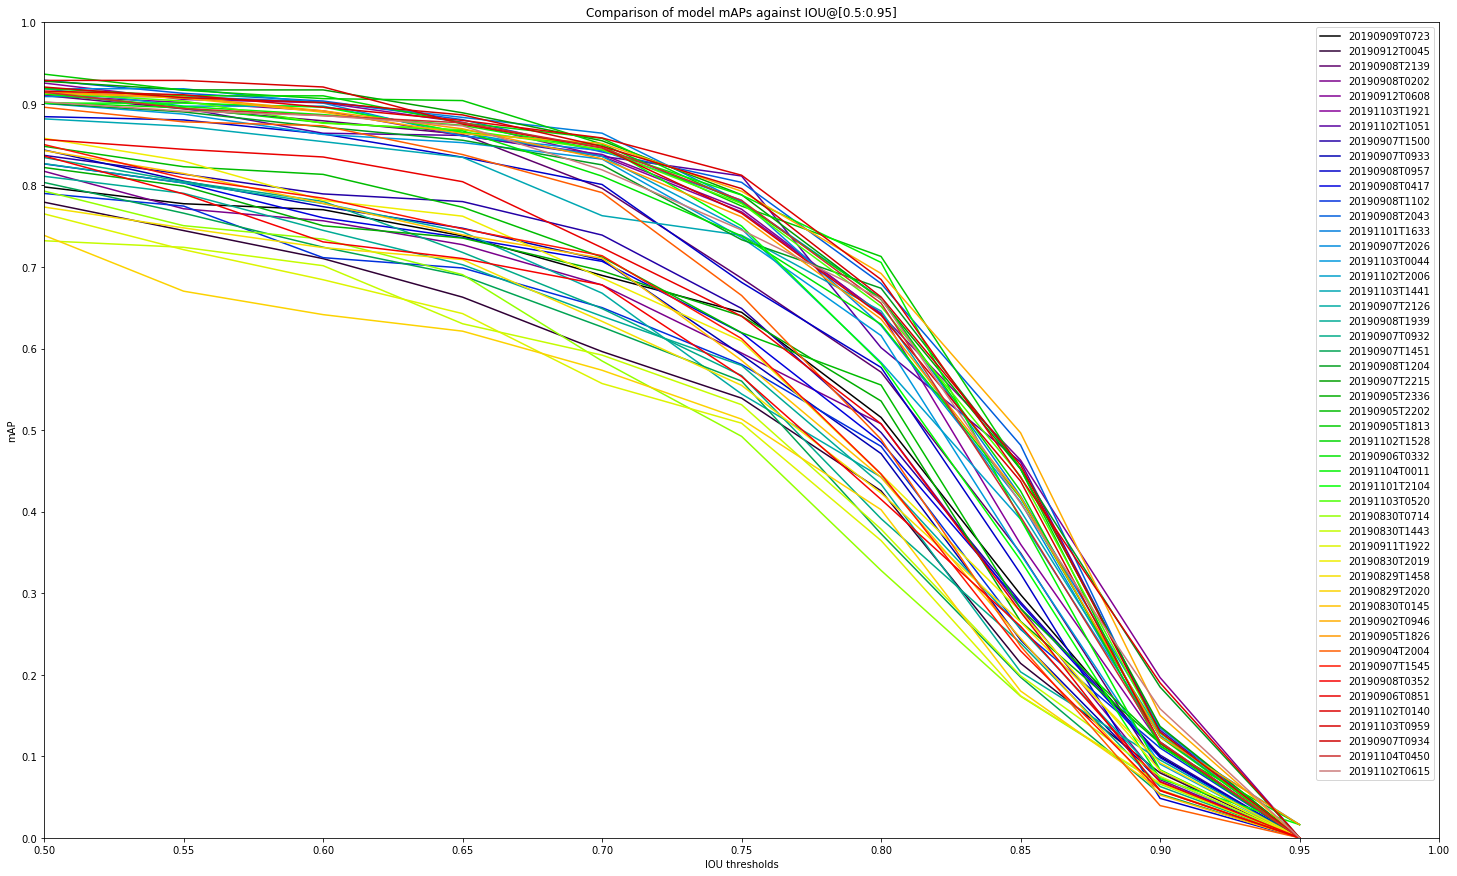
\includegraphics[scale=0.33]{Chapter3/figs/comparison_graph_all_diff_colours.png}
	\end{center}
	\caption{mAP@IOU[0.5:0.95] scores for all models train in the Mask-RCNN Zanzibar dataset grid search. See Table \ref{tab:MaskRCNNHyperparamTuningGridSearch} for each model's hyperparameters.}
	\label{fig:mAP-graph}
\end{figure}

Whilst Figure \ref{fig:mAP-graph} provides some indication of overall model training, using it to determine the most appropriate model for the task at hand is difficult given the number of models trained. To achieve this, the list of models was reduced to only those which achieved the best mAP@IOU[0.5, 0.75, 0.85] scores. The thresholds 0.5 and 0.75 were chosen as these are often cited in segmentation literature \cite{bolya_190402689_2019, wang_solov2_2020, tian_fcos_2019}. The 0.85 threshold was chosen as some models trained still achieve impressive results here, allowing for further filtering of the models. 

When filtering, the top five performing models at each threshold were extracted and then combined into one list. If a model top five at multiple thresholds it was only included in the list once, resulting in a list of ten best performing models. The mAP@IOU[0.5, 0.75, 0.85] scores for these best performing models can be seen in Figure \ref{fig:mAP-best-models-bar-chart}.

\begin{figure}[h]
	\begin{center}
		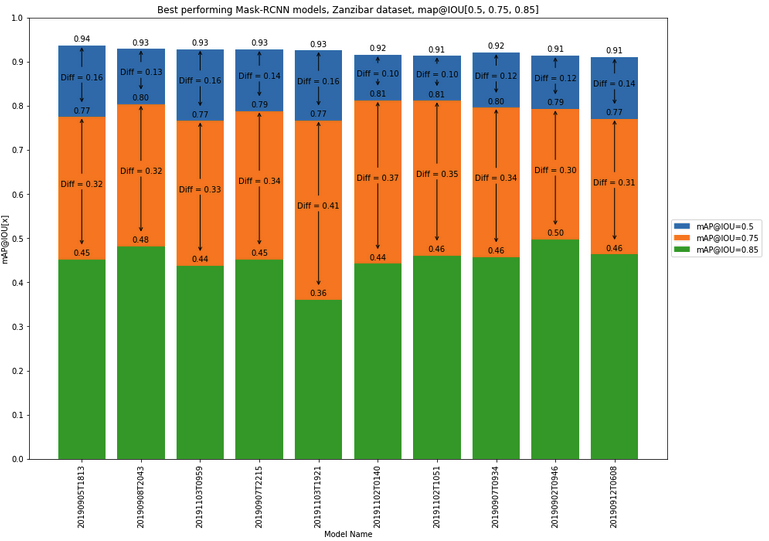
\includegraphics[scale=0.6]{Chapter3/figs/mask-RCNN-model-bar-chart.png}
	\end{center}
	\caption{mAP@IOU[0.5, 0.75, 0.85] scores for the best performing Mask-RCNN models trained on the Zanzibar dataset. See Table \ref{tab:MaskRCNNHyperparamTuningGridSearch} for each model's hyperparameters.}
	\label{fig:mAP-best-models-bar-chart}
\end{figure}

When deciding on which model hyperparameters are best for the task of cetacean segmentation, it is important to find a model with a high mAP@IOU[0.85] score. As the model will be used to perform segmentation before fine-grained classification, it is important the model is capable of removing as much background from the segmentation as possible. Any background included in the segmentation may adversely effect the photo-id process. Using this as criteria, model 20190902T0946 was selected as the best performing model. The model achieves a mAP@IOU[0.85] score of 0.5, an excellent score given the difficulty of the segmentation task. The model also performs well a the other evaluation thresholds, achieving mAP@IOU[0.5, 0.75] scores of 0.91 and 0.79 respectively. These scores verify the model is capable of segmenting the cetacean's fin from the background with as little noise being included in the segmentation mask as possible.

An interesting point to note here is that 20190902T0946 did not achieve the highest mAP@IOU[0.5, 0.75] scores. As previously mentioned, these thresholds are often the ones included in segmentation literature to evaluate model performance. If just these thresholds were used for model selection, 20190902T0946 would not have been chosen. This highlights the need to select models based on metrics which make sense for the task at hand. As the model is required to remove as much background noise as possible, using a high threshold for evaluation makes sense. Thresholds higher than 0.85 were not utilised due to the low performance of all models at this threshold, although 20190902T0946 also achieves the best map@IOU[0.9] score of 0.150. Only one model, 20191102T0615 achieves a better score at this threshold, 0.158, however this model achieves lower performance at the chosen evaluation thresholds of 0.5, 0.75, and 0.85.

\subsection{An Evaluation of Optimal Model Hyperparameters}\label{ch:cetDet,sec:ModelSelection,sub:OptimalHyperparameters}

As discussed in Section \ref{ch:cetDet,sec:ModelSelection,sub:ModelSelectionBasedOnGridSearch} a filter of the trained Mask-RCNN models was performed to determine the best model hyperparameters for the task of cetacean instance segmentation, with model 20190902T0946 being selected. This model's hyperparameters, along with those of the other nine best performing models, can be seen in Table \ref{tab:best-mask-rcnn-models}.

\begin{table}[!ht]
	\tiny
	\begin{adjustbox}{width=\columnwidth, center}
		\begin{tabular}{cccccc}
			\toprule
			Model Name & Weight Decay &        RPN Anchor Scales & Optimiser & Augmentation Strategy & Pre-trained on MSCOCO? \\
			\midrule
				20190902T0946 &         0.01 &   (16, 32, 64, 128, 256) &      SGDR &                  aug1 &                  False \\
				20190905T1813 &        0.001 &  (32, 64, 128, 256, 512) &      SGDR &                  aug1 &                  False \\
				20190907T0934 &         0.01 &  (32, 64, 128, 256, 512) &      SGDR &                  None &                  False \\
				20190907T2215 &        0.001 &   (16, 32, 64, 128, 256) &      SGDR &                  aug2 &                  False \\
				20190908T2043 &       0.0001 &  (32, 64, 128, 256, 512) &      SGDR &                  aug1 &                  False \\
				20190912T0608 &       0.0001 &   (16, 32, 64, 128, 256) &      SGDR &                  aug1 &                  False \\
				20191102T0140 &         0.01 &  (32, 64, 128, 256, 512) &      SGDR &                  aug1 &                  False \\
				20191102T1051 &       0.0001 &   (16, 32, 64, 128, 256) &      SGDR &                  None &                  False \\
				20191103T0959 &         0.01 &  (32, 64, 128, 256, 512) &      SGDR &                  aug2 &                  False \\
				20191103T1921 &       0.0001 &   (16, 32, 64, 128, 256) &      SGDR &                  aug2 &                  False \\
			\bottomrule
		\end{tabular}
	\end{adjustbox}
	\caption{Hyperparameters of the best performing Mask-RCNN models on the Zanzibar dataset. Subset of Table \ref{tab:MaskRCNNHyperparamTuningGridSearch}.}
	\label{tab:best-mask-rcnn-models}
\end{table}





%%%%%%%%%%%%%%%%%%%
\nomenclature[z-CNN]{CNN}{Convolutional Neural Networks}
\nomenclature[z-CV]{CV}{Computer Vision}
\nomenclature[z-CPU]{CPU}{Central Processing Unit}
\nomenclature[z-GPU]{GPU}{Graphical Processing Unit}
\nomenclature[z-SGD]{SGD}{Stochastic Gradient Descent}
\nomenclature[z-ReLU]{ReLU}{Rectified Linear Unit}
\nomenclature[z-FCN]{FCN}{Fully Convolutional Network}
\nomenclature[z-RPN]{RPN}{Region Proposal Network}
\nomenclature[z-SGDR]{SGDR}{Stochastic Gradient Descent with Restarts}
\nomenclature[z-VM]{VM}{Virtual Machine}
